\chapter{Multi-Input Deep Neural Network in Fashion News Popularity Prediction}
\label{exp2}

\begin{quote}
This chapter proposes a new deep learning model with two input layers to predict the fashion news popularity. The preprocessing of the deep learning model is introduced in detail. In addition, the techniques used in the model, including dropout, pooling, and bidirectional gate recurrent unit are discussed. This experiment further shows the prediction performance compared with four state-of-the-art model.
\end{quote}

\section{Data Used}
\label{dl_data}
In this experiment, we use similar dataset in experiment 1. The difference is that, as we do not use concept drift detection framework, we split the dataset into three parts. The fashion news from 1/04/2018 to 13/06/2018 are used as the test dataset. The dataset containing fashion news from 01/01/2014 to 31/03/2018 is split randomly into two subset. The subset containing 90\% news is used to training the model and the subset containing rest 10\% news is responsible to tune the hypeparameters. The number of examples in each dataset and the proportion of each class is shown in Table \ref{prop} 

\begin{table}[]
\centering
\begin{tabular}{c|cccl}
\multirow{2}{*}{Dataset} & \multirow{2}{*}{Number of news} & \multicolumn{3}{c}{Proportion of class} \\
                         &                                 & Hot         & Medium      & Cold        \\ \hline
Trian                    & 74996                           & 0.0721      & 0.3794      & 0.5485      \\
Validation               & 8333                            & 0.0728      & 0.3760      & 0.5512      \\
Test                     & 4188                            & 0.1445      & 0.3677      & 0.4878     
\end{tabular}
\caption{Properties of the datasets}
\label{prop}
\end{table}

To characterize the text classification problem and help tune the hypeparameters, the number of words in a sample from training set is collected and shown in Table \ref{num_words}


\begin{table}[]
\centering
\begin{tabular}{c|ccc}
\multirow{2}{*}{} & \multicolumn{3}{c}{Number of words per sample} \\
                  & Median        & Maximum        & Average       \\ \hline
Text              & 114           & 6258           & 158.59        \\
Title             & 19            & 59             & 19.60         \\
Keywords          & 3             & 36             & 3.24         
\end{tabular}
\caption{Number of words per sample}
\label{num_words}
\end{table}


\section{Model Design and Implementation}
This section introduces the preprocessing of the raw data which is shown in Figure \ref{dl_preprocess}. Then, the structure of the model is discussed. As shown in Figure \ref{dl_structure}, the model proposed in this section contains two parts. The first part receives the unigram and bigram of the keywords and title as the input. The architecture of this part is similar to fastText model which uses a word embedding layers that maps each word in the input into a low dimension word vector. Then, the word vectors is averaged to produce a sentence-level representation. The second part received the preprocessed text and also produce the word vectors by an embedding layer. The difference is that a bidirectional GRU is applied to model the word sequence and output the word-level representation. Then both a max pooling layer and an average pooling layer are used to merges the word-level representations. The sentence-level features are produced by concatenate the outputs from these two pooling layers. Finally, the prediction result is given by the fully connected layers.

The basic idea behind this model is that the order of the words and the long distance pattern is important for modeling the text but unimportant for modeling the titles and keywords. The word distribution is feature that we expect to extract from the keywords and titles. Thus, we design two different feature extractors, one inspired by fastTex focus on the word vectors and one similar to BLSTM~\cite{zhang2015relation} uses RNN component to extract the long distance pattern. These components will be discussed in detail in this section.


\subsection{Preprocessing}
\begin{figure}
\centering
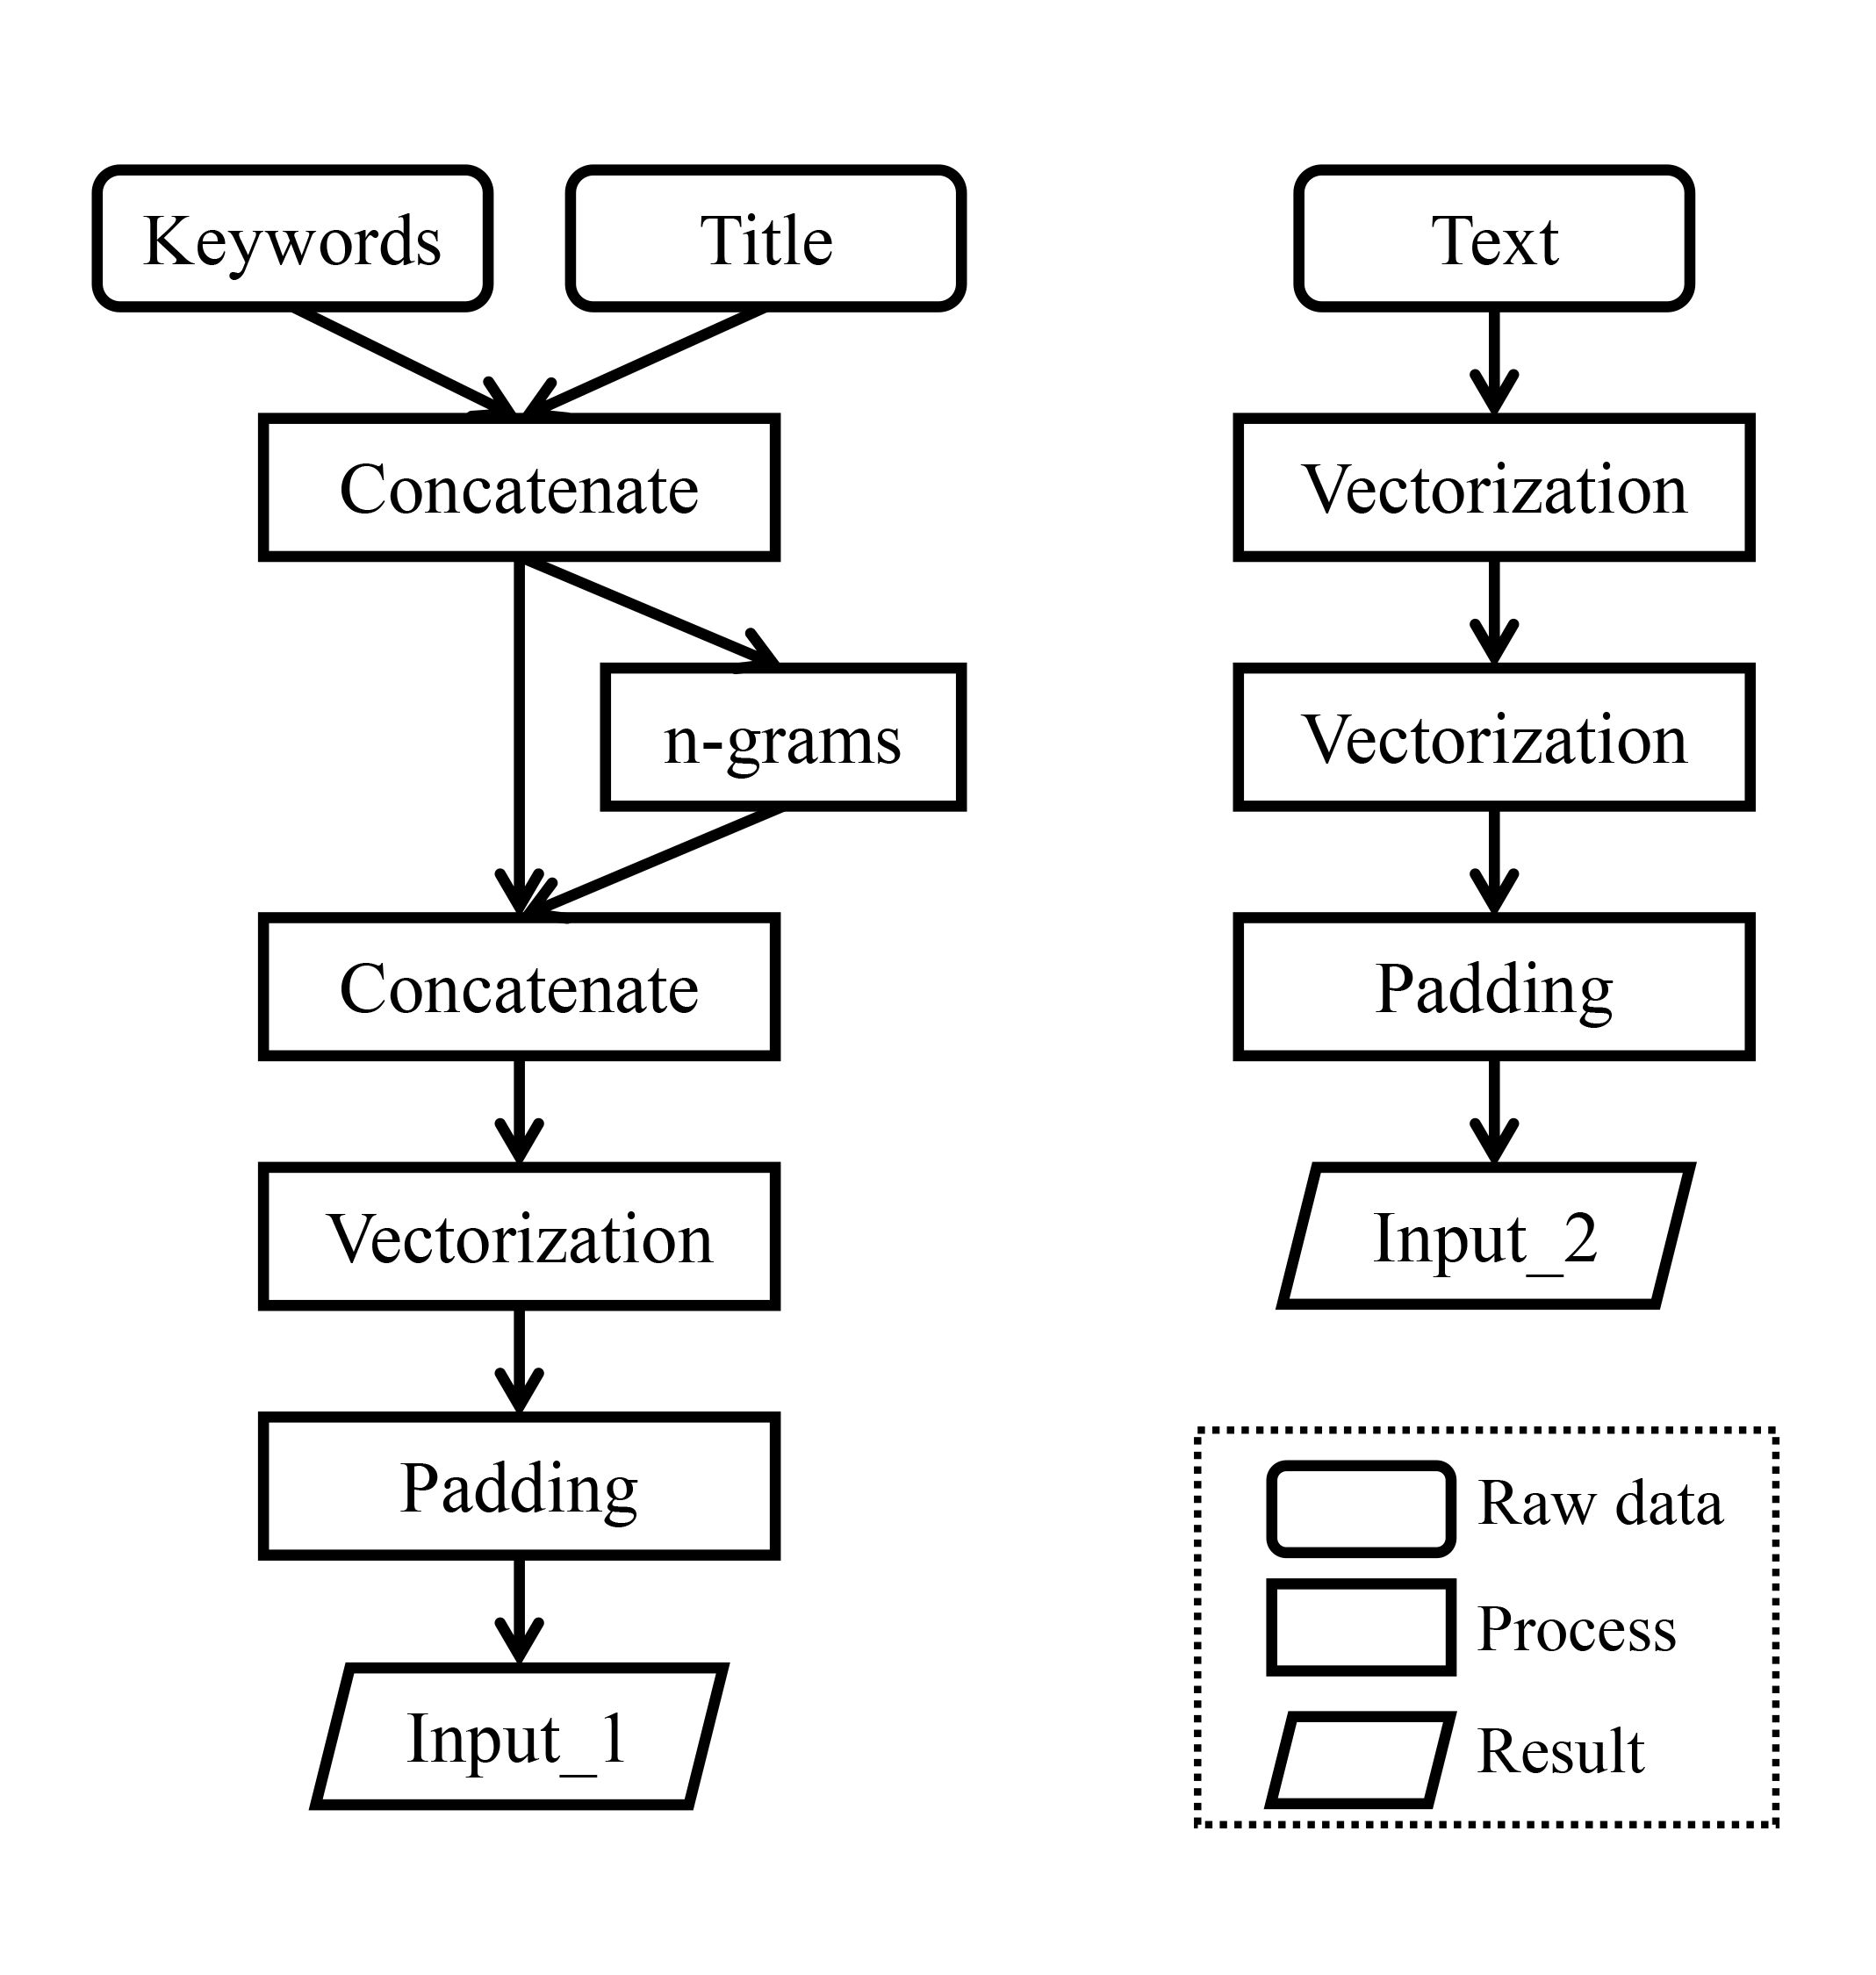
\includegraphics[width=0.6\textwidth]{dl_preprocess.png}
\caption{Preprocessing of the deep learning model}
\label{dl_preprocess}
\end{figure}

The procedure of the preprocessing for keywords, title, and text is shown in Figure \ref{dl_preprocess}. 

In a sample, the keywords and title are concatenate to a new sentence. Though the long distance pattern of this new sentence is not the one of the features we want, it is useful to capture some participial information about the local word order. Thus, the bag of n-grams is used as the additional feature. Considering the efficiency and most of keywords that are composed of two or fewer words, we use a bag of bigrams to keep the partial information. After this process, the sentence is represented as a sequence of unigrams and bigrams. Then the sequence is turned into numerical vector. A unique index is assigned to each unigram and bigrams. As keywords and title are the information extracted from the text, we keep all the words in our vocabulary.

However, not all words in the text contribute to the popularity predictions. In the process of tokening the text, the text is represented as a sequence of the unigrams and some rare and irrelevant words are discards from the vocabulary. In the experiment, we observe that using the most frequent 20,000 features is generally sufficient. 

The final step for two inputs is the padding. Sequences that are shorter than max length are padded with $0$ at the end while sequences longer than max length are truncated. In the experiment, the max length of the sequence is defined by the median number of words in each element. As shown in Table \ref{num_words}, the max length for title and keywords is sequence is $22$ and that for text is $114$.

\begin{figure}
\centering
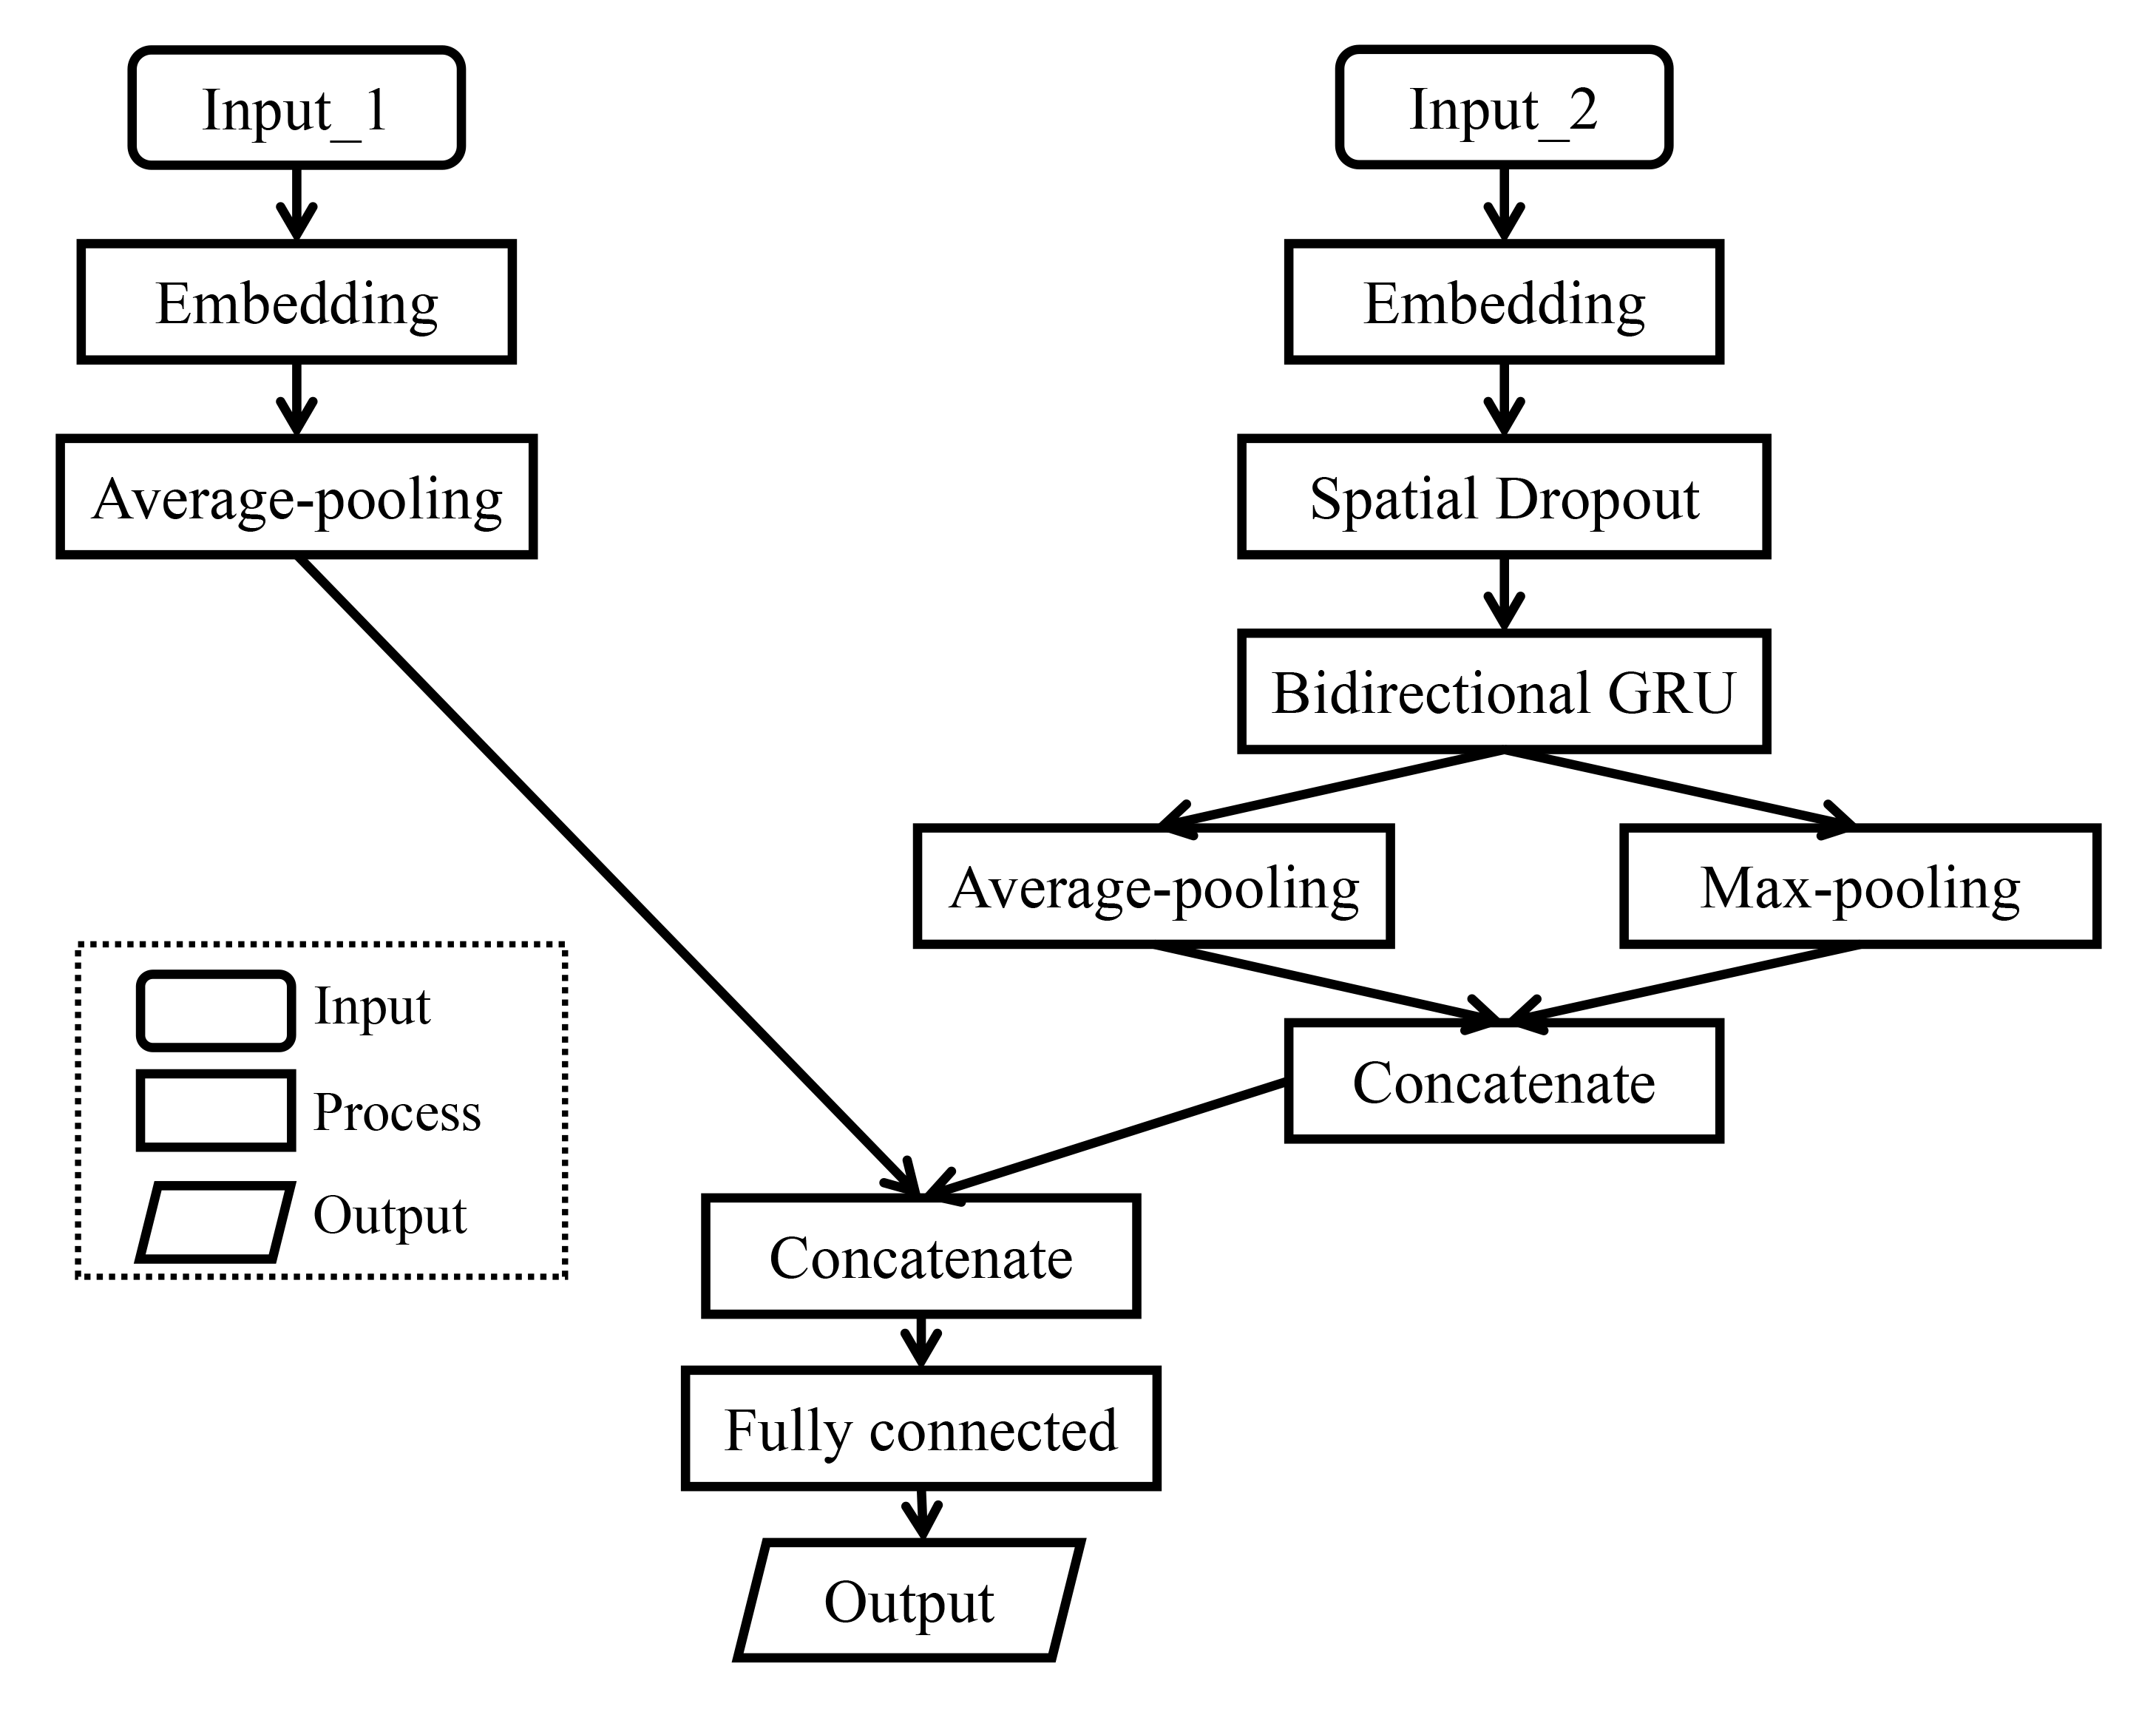
\includegraphics[width=0.8\textwidth]{dl_structure.png}
\caption{Structure of multi-input deep learning model}
\label{dl_structure}
\end{figure}
\subsection{Word Embeddings}
The first component of the proposed model is the word embedding layers. Both inputs are projected to low-dimensional word vectors by the embedding layers. After that, each word gets mapped to a dense vector of real values representing that word's location in semantic space. The advantage of using word vector is that the location and distance between vectors indicates how similar they are semantically. 

A sequence of $n$ indexes, where $n$ is the max length of the input which defined at the process of padding, is firstly transfered to one-hot encoding matrix $\mathbf{X}$. Let $\mathbf{X} \in \{1,0\}^{n \times V}$ where $V$ denotes the size of the vocabulary. The embedding layer transfers the one-hot encoding matrix into matrix containing composed of word vectors as follows
\begin{equation}
\mathbf{E} = \mathbf{X} \mathbf{W}
\end{equation}  

where $\mathbf{W} \in \mathbb{R}^{V\times D}$ and $D$ is the dimension of the word vector. Since $\mathbf{X}$ is one-hot, $\mathbf{W}$ is actually stores representations of all the words in the vocabulary.

There are two approach to initialize the projection weight $\mathbf{W}$. One is random initialization which will be updated during the training process. Another is using the pre-trained word vectors, by which the knowledge of general domains can be used. In our research, the embedding layer for the title and keywords is initialized randomly. Because, the keywords contains many celebrities' name, such as A\$AP Rockey, Young Nudy, and brands, such as YEEZY, Suicoke, which are not commonly used words so that the pre-trained word vectors do not contain these words. The dimension of the word vectors is set to $20$ as suggested by Joulin~\cite{Joulin2016}.

In contrast, the embedding layer for the text is initialized by the pre-trained weight. In order to compare with the work by Zhang~\cite{zhang2015relation} and Zhou et al.~\cite{zhou2016attention}, the model uses the same word vectors proposed by Turian et al. ~\cite{turian2010word}, which are 50-dimensional, to initialize the projection matrix.


\subsection{Bidirectional Gated Recurrent Unit Neural Networks}
\begin{figure}
\centering

\includegraphics[width=0.7\textwidth]{gru.png}
\caption{Graphical illustration of the GRU~\cite{Chung2014}.}
\label{GRU}
\end{figure}

The second component of the model is the bidirectional recurrent layer which is the key component for modeling the sequence and capture the long-distance pattern. 

We start from the gated recurrent unit(GRU). LSTM and GRU are both the variations of the RNN. But GRU can also be considered as a variation on the LSTM. The mechanism of the LSTM is introduced in Section \ref{background_lstm}. One of the difference between these two units is that GRU only has two gates which controls the information flow inside the units, however, without having an output gate that controls the exposure of the outputs. Another difference is the location of the input gate (reset gate). GRU controls the information from the previous activation when computing the new activation while LSTM controls it independently.

We assume $\mathbf{h}_t$ is the activation at time $t$ of the GRU, which is defined as follow
\begin{equation}
h_t^j = (1-z_t^j) h_{t-1}^j + z_t^j \hat{h}_t^j
\end{equation}
where $\mathbf{h}_{t-1}$ is the previous activation, $\hat{\mathbf{h}}_t$ is the candidate activation, and $\mathbf{z}_t$ is the update gate which controls how much of the past information needs to be passed along to the future. The update gate is computed by 
\begin{equation}
z_t^j = \sigma(W_z \mathbf{x}_t + U_z \mathbf{h}_{t-1})^j 
\end{equation}
In addition, the candidate activation $\hat{\mathbf{h}}_t$ is computed by the equation which is similar to the traditional recurrent unit. 
\begin{equation}
\hat{h}_t^j = \mbox{tanh}(W \mathbf{x}_t + U(\mathbf{r}_t \odot \mathbf{h}_{t-1}))^j
\end{equation}

where $\mathbf{r}_t$ is the reset gate which controls how much of past information flow to forget. Its computation is similar to the update gate 
\begin{equation}
r_t^j = \sigma(W_r \mathbf{x}_t + U_r \mathbf{h}_{t-1})^j
\end{equation}

As we discussed in Section \ref{background_lstm}, the problem of the one-directional forward RNN is that the information of the future vectors are not fully utilized. Thus, we use the bidirectional architecture to extract the features from both past words and future words. The graphic illustration of bidirectional LSTM is shown in Figure \ref{blstm}. The bidirectional GRU is same to bidirectional LSTM, just change the type of the unit. Zhang~\cite{zhang2015relation} and Zhou et al.~\cite{zhou2016attention} both summed the outputs from forward and backward. In order to retain as much information as possible, we concatenate the outputs from both directions. 

In the experiment, the  size of the GRU unit is set to 80. 

\subsection{Pooling Layer}
The third component of our model is the pooling layer. In the experiment, we use two types of pooling layers. The objective of using pooling layer is compress the word-level representations to sentence-level feature vectors. One of the compression method is the accumulation approach which use the feature vector produced at the last time step from RNN layer. However, we use the bidirectional RNN which can not defined what is last time step. Thus, most of RNN models resort to the pooling approach as in CNN models. 

However, different from the pooling layer used in CNN models which specify the kernel size of the pooling layer, the pooling layer in RNN are mostly the global pooling. In our research, the global max-pooling and global average-pooling are defined as follows:
\begin{equation}
m_i = \mbox{max}_t\{(h_t)_i\}
\end{equation}
\begin{equation}
m_i = \mbox{average}_t\{(h_t)_i\}
\end{equation}
where $m$ is the sentence-level feature vector and $i$ indexes features dimensions~\cite{zhou2016attention}. 

For title and keywords, we use the global average pooling which is suggested by ~\cite{Joulin2016}. For the text, the novelty is that we use two pooling methods and the sentence-level representation is produced by concatenating the outputs from the pooling layers. The hypothesis is that some keywords play important a role in prediction but the overview of the sentence is also very important. So max-pooling extracts the keywords information while average-pooling provides the overview of the sentence.


\subsection{Classifying}
The sentence-level feature vectors from title\&keywords and text are concatenated and passed to the final classifier. In the experiment, the fully connected neural network is classifier and softmax function is used to predict the label. For the concatenated feature vector $\mathbf{h}^* \in \mathbb{R}^{d}$, the prediction is given by
\begin{equation}
\mathbf{J} = W_j \mathbf{h}^* + b_j
\end{equation}
\begin{equation}
\hat(p)(y|S) = \mbox{softmax}(W_S \mathbf{J} + b_S)
\end{equation}
\begin{equation}
\hat{y} = \mbox{argmax}_y \hat{p}(y|S)
\end{equation}
where $W_j, b_j$ is the weights of the fully connected layer and $W_S, b_S$ is the weights of the output layer. 

As our dataset is very imbalance, traditional cost function, such as negative log-likelihood, does not punish the majority class. To solve this problem, we resort the focal loss in image classification. Focal loss was proposed by Lin et al. for dense object detection~\cite{Lin2017}. The definition of the focal loss can address the class imbalance by down-weighting the loss assigned to well-classified examples. 

We assume $t\in \mathbb{R}$ is the ground truth, $p_t$ is defined as 
\begin{equation}
p_t = \hat{p}(t|S)
\end{equation}

The focal loss is defined as 
\begin{equation}
\mbox{FL}(p_t) = -(1-p_t)^\gamma \mbox{log}(p_t)
\end{equation}

where $\gamma$ is the focusing parameter adjusting the rate at which easy examples are down-weighted. And when $\gamma = 0$, FL is equivalent to cross entropy. Focal loss shows its advantage when $p_t \rightarrow 1$. $(1-p_t)^\gamma$ goes to $0$ by which the easy example is down-weighted.


\subsection{Regularization}
We punish the complex model by adding an additional dropout layer after embedding layer. The role of dropout layer is preventing the activations from becoming strongly correlated so that the generalization of the model can be approved. It is an effective regularization method in deep learning model.

Instead of using standard dropout, we apply the spatial dropout to our model. The standard dropout set individual `pixel' to $0$randomly, which works well on images because adjacent pixels are highly correlated. However, the correlation between the feature vectors are more important on texts. Thus, Spatial dropout randomly omits the entire feature maps by setting them to $0$, which works better in our model~\cite{tompson2015efficient}.

In the experiment, the dropout rate is set to $0.2$, which indicates 20\% of the word vectors will be dropped.

\subsection{Evaluation Metrics}
The evaluation metrics in this experiment is similar to the experiment 1, including accuracy, macro-F1, macro-Recall, and the confusion matrix. The difference is that we use Area Under the macro averaged Receiver Operating Characteristic Curve (ROC AUC) score to evaluate the prediction performance.

A ROC curve is a graphical plot that illustrate the prediction ability of a binary classifier. The x-axis of the curve is the false positive rate (FPR) with different threshold. The FPR is defined as 
\begin{equation}
\mbox{FPR} = \frac{fp}{fp+tn}
\end{equation}
where $fp$ is number of positive instances which are incorrectly predicted, and $tn$ is the number of negative instances which are correctly predicted. The y-axis of the curve is the true positive rate (recall) with different threshold. 

ROC AUC score is obtained by computing the area under the ROC curve. ROC AUC store is 1 indicating perfect classifier and between 0 to 1 indicating the classifier is better than random guess. 

The definition of macro averaged ROC AUC score is same to macro-F1 and macro-Recall introduced in Section \ref{cd_metrics}, which calculates the metrics for each label and outputs the unweighted mean.

\subsection{Model Training}
The model is trained by training dataset and 
validated by the validation dataset, which described in Section \ref{dl_data}. The focal loss function is optimized by Adam optimization algorithm~\cite{Kingma2014}. Adam combines the advatanges of adaptive gradient algorithm (AdaGrad) and root mean square propagation (RMSProp) which can handle sparse gradients on noisy problem. In the training process, the Adam algorithm is applied with learning rate of 0.1 and mini batch size of 32.

To prevent overfitting and find the best model, the validation-based early stopping technique is used in the training process. 
At the end of each epoch, the ROC AUC score on validation dataset will be computed and the current weights of the model will be stored. In the experiment, the patience of the early stopping is set to $5$. After 5 epochs with no improvement of the ROC AUC score, the training will be stopped. The best model will be selected from the stored model with the highest ROC AUC score. 

In addition, except for the embedding layer for text inputs which is initialized with pre-trained word vectors, all the weights are initialized randomly. 

\subsection{Comparison Models}
Recently, a variety of the deep learning model have been applied to text classification. We choose four stat-of-the-art and representative models for comparison. These four models have different functional components and mechanisms which are discussed in Section \ref{dl}.

\textbf{fastText.} fastText only uses an embedding layer to extract word vectors and an global average pooling layer to produce sentence-level representation. It is a fast and effective classification model which widely used as a baseline model. The parameters of used in comparison is same to the model described in the original paper ~\cite{Joulin2016}. The embedding layer is initialized randomly and the dimension of the word vector is set to $20$. The inputs the sequence concatenating the title and text.

\textbf{Character-level Convolutional Network}
The char-level CNN is only one comparison model whose functional layer is the convolutional layer. The advantage of the char-level CNN is that it has very high fault tolerance. As it classify the text in character level, it can easily deal with the typos or the unseen words. The model structure used in comparison is same to what is described in Table \ref{config_char_cnn} and Table \ref{config_char_fl}. We use the same low-case alphabet presented in Section \ref{cnn_background}.

\textbf{Bidirectional Long-Short Term Memory Network.}
The BLSTM used in comparison is the model introduced in Section \ref{background_lstm}. The size of LSTM unit is set to $256$ as suggested by the author. To ensure fair comparison, the embedding layer is initialized with the same pre-trained word vectors proposed by Turian et al. ~\cite{turian2010word}. The model is trained by stochastic gradient descent algorithm. 

\textbf{Attention Based Bidirectional Long Short-Term Memory Network.}
The Att-BLSTM has same bidirectional RNN layer with BLSTM. In addition, its embedding layer is also initialized with the Turian's pre-trained weights. The difference is that Att-BLSTM is trained by AdaDelta and regularized the model parameters with L2 regularization strength of $10^{-5}$.



\section{Experimental Results}
